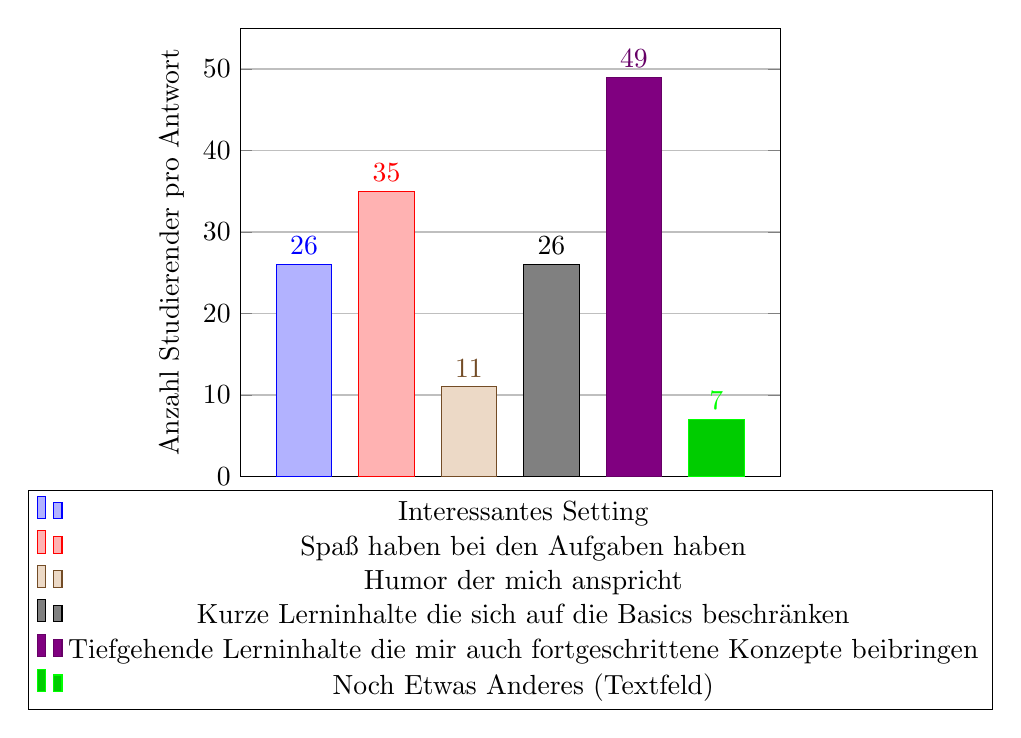
\begin{tikzpicture}
    \begin{axis}[
        x tick label style={
    		/pgf/number format/1000 sep=},
    	ylabel=Anzahl Studierender pro Antwort,
    	enlarge x limits=2,
        ymax=55,
        ymin=0,
    	legend style={at={(0.5,-0.03)},
        anchor=north,legend columns=1},
        ybar,
        bar width=20pt,
        xticklabels={},
        xtick=\empty,
        nodes near coords,
        grid=major,
    ]
    \addplot coordinates {(1,26)};
    \addplot coordinates {(2,35)};
    \addplot coordinates {(3,11)};
    \addplot coordinates {(4,26)};
    \addplot coordinates {(5,49)};
    \addplot coordinates {(6,7)};
    
    \legend{Interessantes Setting, Spaß haben bei den Aufgaben haben, Humor der mich anspricht, Kurze Lerninhalte die sich auf die Basics beschränken, Tiefgehende Lerninhalte die mir auch fortgeschrittene Konzepte beibringen, Noch Etwas Anderes (Textfeld)}
    \end{axis}
    \end{tikzpicture}